\documentclass[border=10pt]{standalone}

\usepackage{tikz}
\usepackage{tikzsymbols}
\usetikzlibrary{calc,patterns,shapes.geometric}

\def\centerarc[#1](#2)(#3:#4:#5){\draw[#1] ($(#2)+({#5*cos(#3)},{#5*sin(#3)})$) arc (#3:#4:#5);}

\begin{document}
	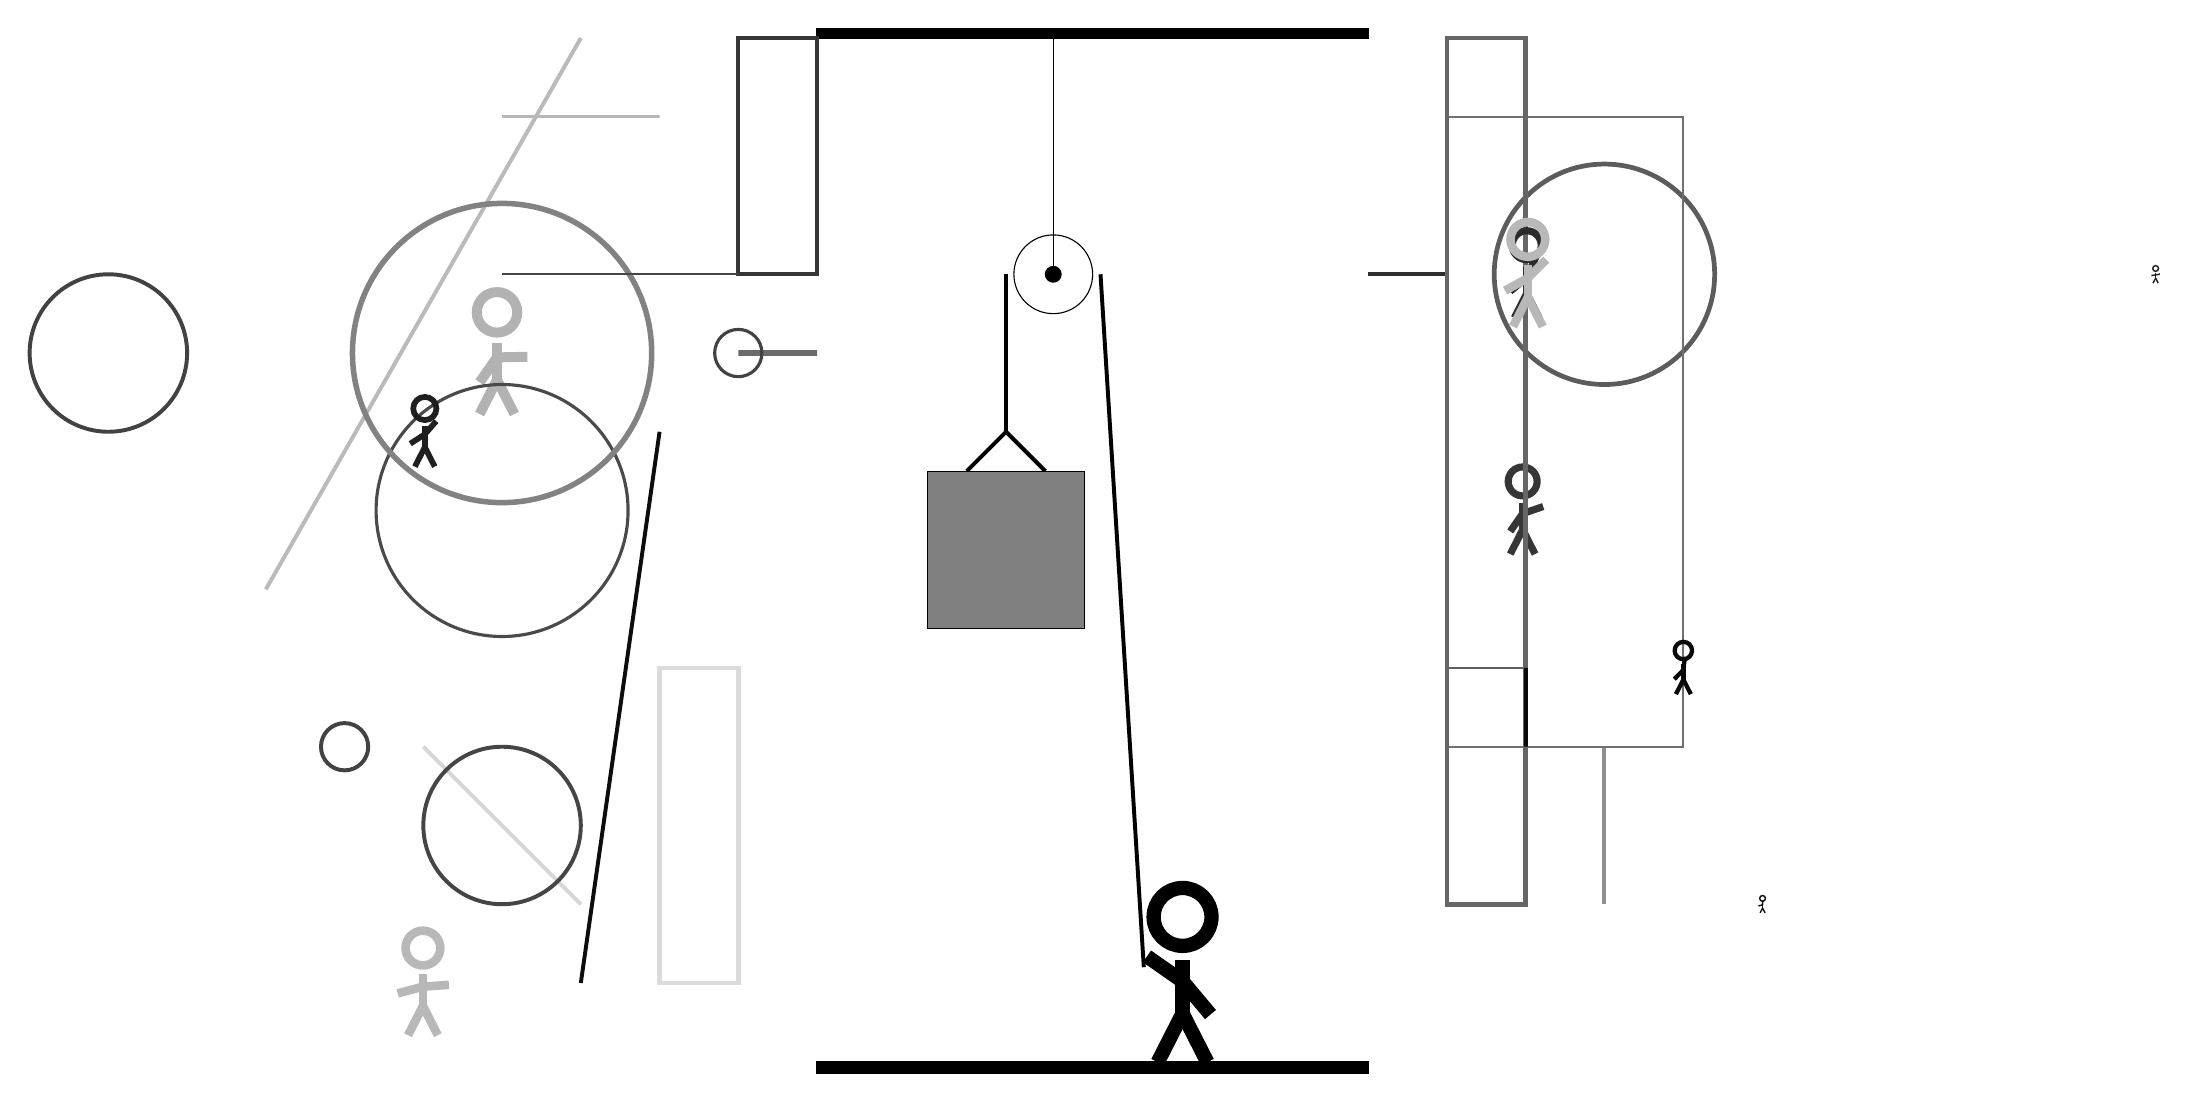
\begin{tikzpicture}
		%%%%% START %%%%%
		
		\draw[fill=black] (-2, 10) rectangle (5, 10.125);
		
		\draw (1, 7) circle (0.5);
		\draw[fill=black] (1, 7) circle (0.1);
		\draw (1, 10) -- (1, 7);
		
		\draw[line width=0.5mm] (-0.1, 4.5) -- (0.4, 5.0) -- (0.9, 4.5);
		\draw[fill=black!50] (-0.6, 4.5) rectangle (1.4, 2.5);
		
		\draw[line width=0.5mm] (0.4, 7) -- (0.4, 5.0);
		\centerarc[line width=0.5mm](1, 7)(0:180:0.6);
		\draw[line width=0.5mm](1.6, 7) -- (2.15, -1.8);
		
		\node at (2.6, -1.9) {\Strichmaxerl[10][-35][-50]};
		
		\node[line width=0.7mm, color=black!79] at (7, 4) {\Strichmaxerl[5][55][19]};
		
		\draw[line width=0.5mm, color=black!95](-4, 5) -- (-5, -2);
		\draw [line width=0.5mm, color=black!74](-8, 1) circle (0.3);
		\draw [line width=0.6mm, color=black!64](8, 7) circle (1.4);
		
		\node[line width=0.4mm, color=black!30] at (-6, 6) {\Strichmaxerl[7][55][1]};
		
		\draw[line width=0.3mm, color=black!63] (7, -1) rectangle (6, 2);
		\draw[line width=0.6mm, color=black!14] (-3, 2) rectangle (-4, -2);
		\draw[line width=0.5mm, color=black!44](8, 1) -- (8, -1);
		\draw [line width=0.4mm, color=black!71](-6, 4) circle (1.6);
		\draw[line width=0.5mm, color=black!27](-5, 10) -- (-9, 3);
		\draw[line width=0.5mm, color=black!82](5, 7) -- (6, 7);
		\draw[line width=0.5mm, color=black!16](-5, -1) -- (-7, 1);
		\node[line width=0.3mm, color=black!28] at (-7, -2) {\Strichmaxerl[6][15][4]};
		
		\draw [line width=0.5mm, color=black!73](-6, 0) circle (1.0);
		\draw[line width=0.5mm, color=black!79] (-2, 7) rectangle (-3, 10);
		\node[line width=0.2mm, color=black!88] at (-7, 5) {\Strichmaxerl[4][33][49]};
		
		\node[line width=0.2mm, color=black!87] at (15, 7) {\Strichmaxerl[1][9][11]};
		
		\draw [line width=0.7mm, color=black!49](-6, 6) circle (1.9);
		\draw[line width=0.7mm, color=black!58] (-2, 6) rectangle (-3, 6);
		
		\draw[line width=0.3mm, color=black!56] (6, 1) rectangle (9, 9);
		\node[line width=0.3mm, color=black!97] at (9, 2) {\Strichmaxerl[3][46][83]};
		
		\draw[line width=0.6mm, color=black!60] (7, 10) rectangle (6, -1);
		\draw[line width=0.5mm, color=black!96] (7, 1) rectangle (7, 2);
		\node[line width=0.5mm, color=black!83] at (7, 7) {\Strichmaxerl[5][40][66]};
		\node[line width=0.4mm, color=black!28] at (7, 7) {\Strichmaxerl[6][29][45]};
		
		\draw[line width=0.2mm, color=black!73] (-3, 7) rectangle (-6, 7);
		\draw [line width=0.4mm, color=black!74](-3, 6) circle (0.3);
		\node[line width=0.6mm, color=black!94] at (10, -1) {\Strichmaxerl[1][15][88]};
		\draw[line width=0.4mm, color=black!28] (-4, 9) rectangle (-6, 9);
		
		\draw [line width=0.5mm, color=black!74](-11, 6) circle (1.0);
		
		\draw[fill=black] (-2, -3) rectangle (5, -3.15);
		
		%%%%% END %%%%%
	\end{tikzpicture}
\end{document}